\documentclass{article}
\usepackage[a4paper]{geometry}
\usepackage[procnames]{listings}
\usepackage{float}
\usepackage{color}
\usepackage{graphicx}
\usepackage{cite}
\usepackage{url}
\usepackage{microtype}

\author{Will Luckin}
\title{Simple Graphing and Data Analysis in Python}

\begin{document}
\definecolor{keywords}{RGB}{255,0,90}
\definecolor{comments}{RGB}{0,0,113}
\definecolor{red}{RGB}{160,0,0}
\definecolor{green}{RGB}{20,20,20}

\lstset{language=Python, 
        basicstyle=\ttfamily\small, 
        keywordstyle=\color{keywords},
        commentstyle=\color{comments},
        stringstyle=\color{red},
        showstringspaces=false,
        identifierstyle=\color{green},
        procnamekeys={def,class}}

\maketitle

\begin{abstract}
  This document serves as a guide for any kind of \texttt{Python}
  based plot that a self-respecting Physicist may have to whip up in
  the course of duty.
  Published at \url{physics.luckin.co.uk}.
\end{abstract}

\tableofcontents
\newpage

\section{Introduction}
This document aims to serve as a guide for simple data analysis, for
Physics, in \texttt{Python, Numpy and Matplotlib}.  

\section{Quick start: Plotting a simple graph}
\subsection{Importing the data}
Firstly, one must open a blank .py file in a suitable editor (GNU
Emacs, Sublime Text 3, etc).

At the head of the \texttt{Python} file, one must import the libraries
we are to use. This allows Python to be used to plot graphs and
analyse data.

\begin{lstlisting}
  import numpy as np
  from matplotlib import pyplot as plt
\end{lstlisting}

Then, the data to be plotted must be inputted into Python. This can
either be in the form of a raw Python list or numpy array, or by
importing an external data file. \footnote{Creating a valid external
  data file is covered in the appendices.}

\begin{lstlisting}
  # simple python flat lists
  x_data = [1, 2, 3, 4, 5]
  y_data = [1, 2, 4, 5, 6]

  # numpy arrays
  x_data = np.array([1, 2, 3, 4, 5])
  y_data = np.array([1, 2, 4, 5, 6])
\end{lstlisting}

Importing external data is slightly more complicated. There are a few
use cases to cover:

\begin{lstlisting}
  # simple, tab-seperated file with no headers
  data = np.loadtxt('file.txt')
  # simple, comma-separated file with no headers
  data = np.loadtxt('file.csv', delimiter=',')
  # tab-seperated file with headers occupying one row
  data = np.loadtxt('file.csv', skiprows=1)
\end{lstlisting}

Any kind of \texttt{ValueError} is most likely due to needing the
\texttt{skiprows} argument to skip column headers. Data imported in
this way, or manufactured as a single Numpy array in Python, will be a
2D array; different columns can be accessed via Numpy's slicing.

\begin{lstlisting}
  # first column
  x_data = data[:, 0]
  # second column
  y_data = data[:, 1]
\end{lstlisting}

\subsection{Rendering the simple plot}
This graph can be simply plotted using \texttt{pyplot}, the easy
interface to \texttt{Matplotlib's} full plotting capabilities. In this
case, to plot a simple line graph, this requires one line.

\begin{lstlisting}
  plt.plot(x_data, y_data)
\end{lstlisting}

To plot a scatter graph instead, replace the word \texttt{plot} with
\texttt{scatter}.

Finally, to actually view this graph, \texttt{pyplot} needs to be told
to actually open a window and render it to the screen. In addition, at
this point a \texttt{png} file of the graph can be saved to the
current working directory.

\begin{lstlisting}
  plt.savefig('graph1.png')
  plt.show()
\end{lstlisting}

This would end up with a plot similar to the following.

\begin{figure}[H]
  \centering
  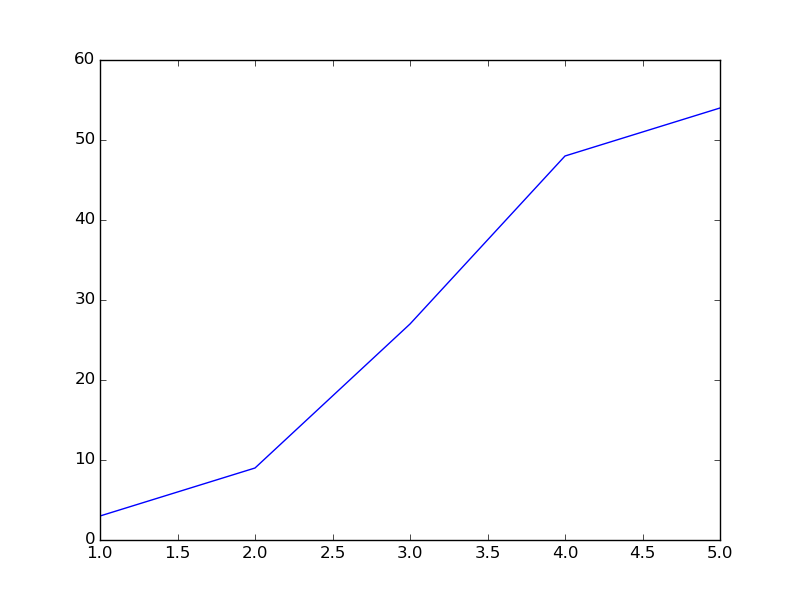
\includegraphics[width=10cm]{ch1.png}
  \caption{A sample, simple plot}
  \label{fig:ch1}
\end{figure}

\subsection{Tidying things up}
Real graphs have axis labels, titles, etc. These are very simple to
add with \texttt{pyplot}. Any mathematical notation must be surrounded
with dollar signs.

\begin{lstlisting}
  plt.title("Example of a graph title")
  plt.xlabel("An x-axis label")
  plt.ylabel("A y-axis label using $LaTeX$ syntax")
\end{lstlisting}

\begin{figure}[H]
  \centering
  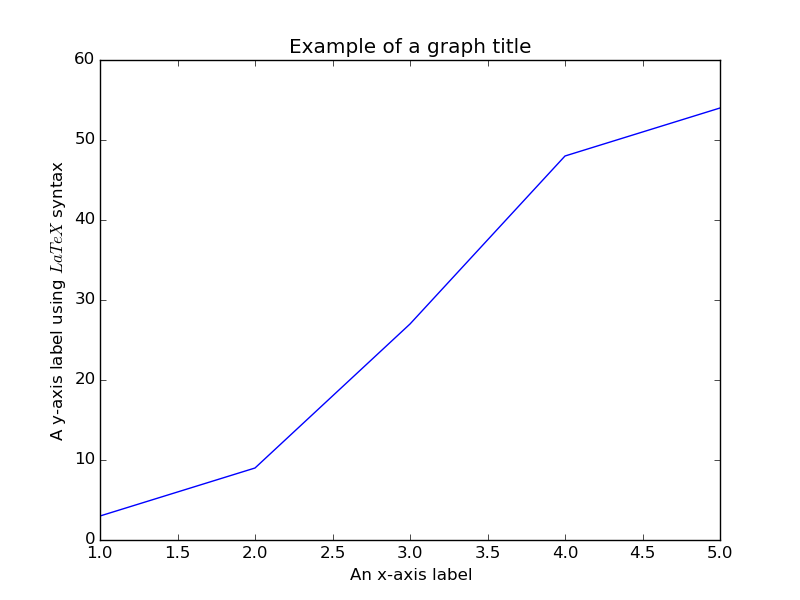
\includegraphics[width=10cm]{ch2.png}
  \caption{Simple plot with axis titles}
  \label{fig:ch2}
\end{figure}

\subsection{Error bars}
Error bars can be added to \texttt{Matplotlib} plots, although it is
somewhat non-trivial due to a few quirks in the library. The key
function here is \texttt{errorbars}. This takes the place of a
\texttt{plt.plot} or a \texttt{plt.scatter}.

\begin{lstlisting}
  plt.errorbars(x_data, y_data, x_err, y_err)
\end{lstlisting}

\begin{figure}[H]
  \centering
  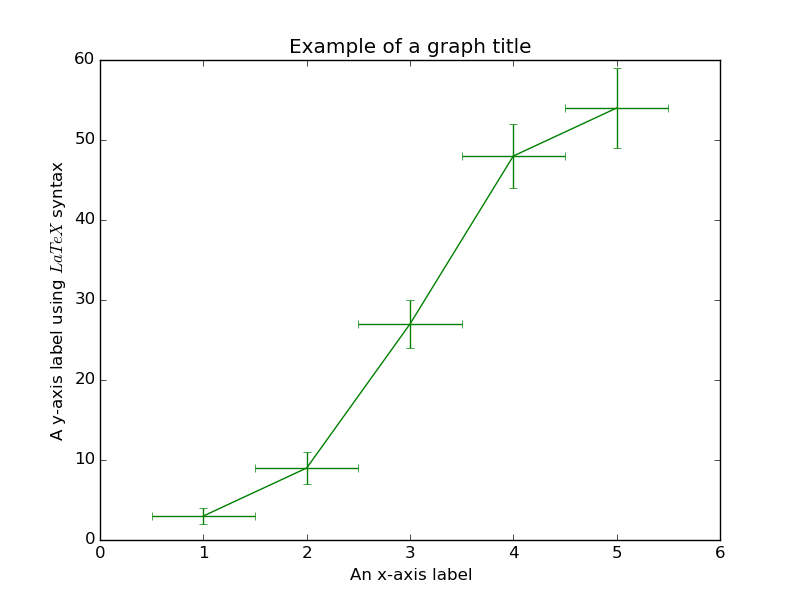
\includegraphics[width=10cm]{ch3}
  \caption{Simple errorbars}
  \label{fig:ch3_1}
\end{figure}

However, this code will automatically plot a line connecting the
data. As this is often not what we want, we can pass in a
\texttt{format string}, or fmt. This string allows the parameters of
the plotted line to be set, and a parameter of \texttt{'o'}
invokes a simple scatter plot.

\begin{lstlisting}
  plt.errorbars(x_data, y_data, x_err, y_err, fmt='o')
\end{lstlisting}

\begin{figure}[H]
  \centering
  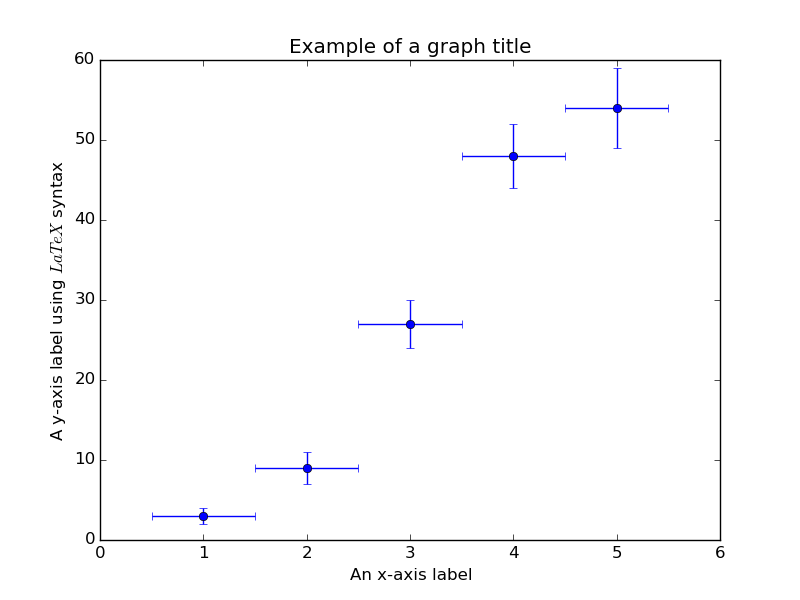
\includegraphics[width=10cm]{ch3_2}
  \caption{Errorbars with a scatter plot}
  \label{fig:ch3_2}
\end{figure}

\section{Fitting a curve to the data}
There are numerous ways to fit a curve to data in the Scipy stack, but
the method explained here is universal, works in every case where you
know the functional form of the data and is quick and simple to
implement. It revolves around a function from the
\texttt{scipy.optimize} submodule, called \texttt{curve\_fit}. This
uses non-linear least-squares fit, to optimise \footnote{Bastardised
  American spellings be damned} a given function to an array of
data. Firstly, therefore, one must prepare this function. You must
know the functional form you wish to fit, but the general principles
are as follows;

\begin{enumerate}
\item Your function must accept the x variable as its first parameter
\item Your function must accept a non-zero amount of additional,
  positional parameters. It cannot accept named parameters.
\end{enumerate}

Before we begin, one must import the fitting function from Scipy:

\begin{lstlisting}
  from scipy.optimize import curve_fit
\end{lstlisting}

Considering the form of a straight line fit as:
\begin{equation}
  \label{eq:slf}
  y = mx + c
\end{equation}

One can translate into \texttt{Python} simply:
\begin{lstlisting}
  def func(x, a, b):
    return a*x + b
\end{lstlisting}

Then, assuming one has arrays of x- and y-data to fit this function
to, the remainder of this follows simply. \texttt{curve\_fit} returns
an array of optimised fit parameters, typically dubbed \texttt{popt},
and the covariance matrix of this fit, typically dubbed \texttt{pcov}.

\begin{lstlisting}
 popt, pcov = curve_fit(func, x_data, y_data) 
\end{lstlisting}

The errors in this fit are wrapped up in the matrix. For an array of
errors, one per each parameter of the fit, one can take the diagonal
elements of the square-rooted matrix.

\begin{lstlisting}
  errors = np.diag(np.sqrt(pcov))
\end{lstlisting}

To plot this fit onto the graph, one can use the simple plotting tools
as covered before, using \texttt{linspace} to generate the range of
$x\_data$. This $x\_range$ is an array of values interpolated between
the minimum and maximum values in the $x$ data. This allows for smooth
plotting of the regression line in the case where the fit is
non-linear.

\begin{lstlisting}  
  popt, pcov = curve_fit(func, x_data, y_data)
  x_range = np.linspace(np.amin(x_data), np.amax(x_data), 100)
  plt.plot(x_range, func(x_range, *popt))
\end{lstlisting}

This would result in the following straight-line fit to the sample
data.

\begin{figure}[H]
  \centering
  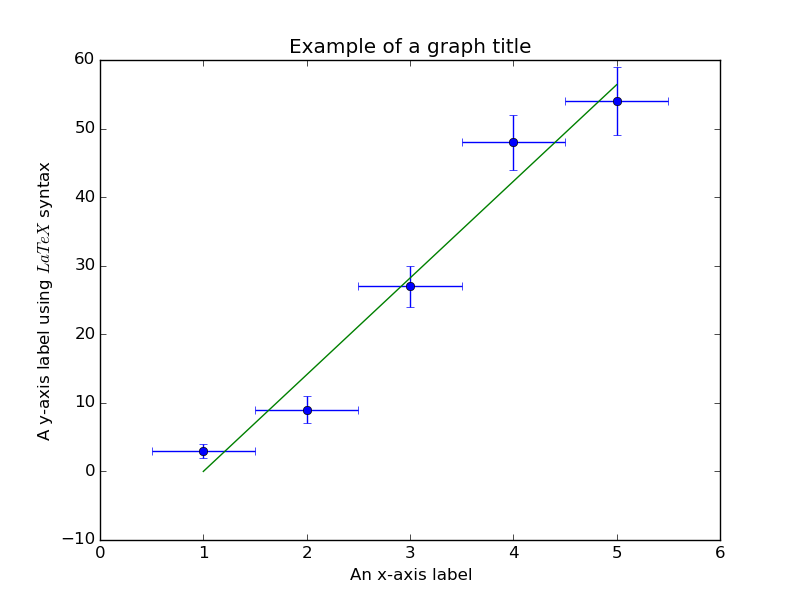
\includegraphics[width=10cm]{ch4}
  \caption{Straight line fit}
  \label{fig:ch4}
\end{figure}

To fit \textbf{any other functional fit} to this data, simply replace
the definition of \texttt{func}. That's all that's required!

\section{More complex plots (unfinished)}
Using the \texttt{pyplot} interface to Matplotlib is a simple way to
create plots, but it makes it difficult to access the more advanced
features that the library offers.

Instead of using the imperitive commands from pyplot and manipulating
the output sequentially, Matplotlib itself uses the object-oriented
abstraction to make it easy to understand and create complex
plots. Before embarking on this, one must understand the terminology
used by Matplotlib.

\begin{description}
\item [Figure] The figure object is the collection of axes, titles,
  etc, that make up your plot. A figure can have multiple axes, but
  each axis belongs to one figure. This is the uppermost level of the
  abstraction. From the Matplotlib website: ``The figure keeps track
  of all the child Axes, a smattering of ‘special’ artists (titles,
  figure legends, etc), and the canvas. (Don’t worry too much about
  the canvas, it is crucial as it is the object that actually does the
  drawing to get you your plot, but as the user it is more-or-less
  invisible to you). A figure can have any number of Axes, but to be
  useful should have at least one.''
\item [Axes] An axes object represents one set of co-ordinate
  axes. This object belongs to a figure. Here, one could set axis
  labels, the background of a specific set of axes, etc.
\item [Line] A line object represents a plotted set of data points on
  an axis. On this object, one can set the colour of the lines, legend
  labels, etc.
\end{description}

Let's begin with a blank Python file, and construct a plot using these
new abstractions, instead of letting pyplot do all the heavy work for
us! In this way, we can get a better understanding of the library, and
therefore understand how to create better and more complicated plots.

Once again, we start by importing all the libraries we shall use:

\begin{lstlisting}
  import numpy as np
  from matplotlib import pyplot as plt
\end{lstlisting}

\section{Appendices}
\subsection{Creating a valid external data file}
This is an incredibly simple process - numpy's \texttt{loadtxt}
function can understand most flat files. The simplest way to get your
data into Python, assuming you don't wish to manually create
multi-dimensional arrays in pure Python is to use spreadsheet
software, such as LibreOffice Calc or Microsoft Excel, and export the
data as a \texttt{Comma Seperated Value, or CSV} file. This can then
easily be loaded into Python, remembering to inform it that you have
values seperated by commas - else it will interpret the entire file as
a single, completely invalid, Python statement!

\begin{lstlisting}
  data = np.loadtxt('mydata.csv', delimiter=',') 
\end{lstlisting}

\end{document}